\documentclass[11pt]{article}\usepackage[]{graphicx}\usepackage[]{color}
%% maxwidth is the original width if it is less than linewidth
%% otherwise use linewidth (to make sure the graphics do not exceed the margin)
\makeatletter
\def\maxwidth{ %
  \ifdim\Gin@nat@width>\linewidth
    \linewidth
  \else
    \Gin@nat@width
  \fi
}
\makeatother

\definecolor{fgcolor}{rgb}{0.345, 0.345, 0.345}
\newcommand{\hlnum}[1]{\textcolor[rgb]{0.686,0.059,0.569}{#1}}%
\newcommand{\hlstr}[1]{\textcolor[rgb]{0.192,0.494,0.8}{#1}}%
\newcommand{\hlcom}[1]{\textcolor[rgb]{0.678,0.584,0.686}{\textit{#1}}}%
\newcommand{\hlopt}[1]{\textcolor[rgb]{0,0,0}{#1}}%
\newcommand{\hlstd}[1]{\textcolor[rgb]{0.345,0.345,0.345}{#1}}%
\newcommand{\hlkwa}[1]{\textcolor[rgb]{0.161,0.373,0.58}{\textbf{#1}}}%
\newcommand{\hlkwb}[1]{\textcolor[rgb]{0.69,0.353,0.396}{#1}}%
\newcommand{\hlkwc}[1]{\textcolor[rgb]{0.333,0.667,0.333}{#1}}%
\newcommand{\hlkwd}[1]{\textcolor[rgb]{0.737,0.353,0.396}{\textbf{#1}}}%

\usepackage{framed}
\makeatletter
\newenvironment{kframe}{%
 \def\at@end@of@kframe{}%
 \ifinner\ifhmode%
  \def\at@end@of@kframe{\end{minipage}}%
  \begin{minipage}{\columnwidth}%
 \fi\fi%
 \def\FrameCommand##1{\hskip\@totalleftmargin \hskip-\fboxsep
 \colorbox{shadecolor}{##1}\hskip-\fboxsep
     % There is no \\@totalrightmargin, so:
     \hskip-\linewidth \hskip-\@totalleftmargin \hskip\columnwidth}%
 \MakeFramed {\advance\hsize-\width
   \@totalleftmargin\z@ \linewidth\hsize
   \@setminipage}}%
 {\par\unskip\endMakeFramed%
 \at@end@of@kframe}
\makeatother

\definecolor{shadecolor}{rgb}{.97, .97, .97}
\definecolor{messagecolor}{rgb}{0, 0, 0}
\definecolor{warningcolor}{rgb}{1, 0, 1}
\definecolor{errorcolor}{rgb}{1, 0, 0}
\newenvironment{knitrout}{}{} % an empty environment to be redefined in TeX

\usepackage{alltt}

\usepackage{amssymb}
\usepackage{amsmath}
\usepackage{bm}
\usepackage{graphicx}
\usepackage{hyperref}
\usepackage{url}
\usepackage{natbib}
\usepackage{epigraph}
\usepackage[utf8]{inputenc} % for UTF-8/single quotes from sQuote()

\usepackage{fancyvrb} % with VerbatimFootnotes, allow verb in footnotes
%\usepackage{listings}
\usepackage{array} % for ragged right table columns
% order of the next two matters
\usepackage[perpage,symbol]{footmisc}
\VerbatimFootnotes

\newcommand{\windows}{\textcircled{w}}
\newcommand{\code}[1]{{\tt #1}}
\newcommand{\flspecific}[1]{\emph{#1}}
%\bibliographystyle{ESA1009}

%\DeclareGraphicsExtensions{.jpg,.pdf,.mps,.png,.bmp}

% \setlength{\textwidth}{6.25in}
% \setlength{\textheight}{8.75in}
% \setlength{\evensidemargin}{0in}
% \setlength{\oddsidemargin}{0in}
% \setlength{\topmargin}{-.35in}
% \setlength{\parskip}{.1in}  
% \setlength{\parindent}{0.0in}  

% \numberwithin{equation}{chapter}
\pagestyle{headings}

\newcommand\R{{\sf R}}
\newcommand\Slang{{\sf S}}
\newcommand{\curRwver}{2013}

\newcommand{\curRver}{3.0.1}

\newcounter{exercise}
\numberwithin{exercise}{section}
\newcommand{\exnumber}{\addtocounter{exercise}{1} \theexercise \thinspace}

\newcommand{\prob}{\text{Prob}}


\sloppy
\title{Matrix models in \R\ (lab 3)}
\author{\copyright 2010 Ben Bolker (modified by Steve Walker)}
\IfFileExists{upquote.sty}{\usepackage{upquote}}{}
\begin{document}

\maketitle

\includegraphics[width=2.64cm,height=0.93cm]{../icons/cc-attrib-nc.png}

\begin{minipage}[b]{3in}
{\small Licensed under the Creative Commons 
  attribution-noncommercial license
(\url{http://creativecommons.org/licenses/by-nc/3.0/}).
Please share \& remix noncommercially,
mentioning its origin.}
\end{minipage}







\section{Basic matrix manipulation}

R uses \code{matrix} to enter matrices:

\begin{knitrout}
\definecolor{shadecolor}{rgb}{0.969, 0.969, 0.969}\color{fgcolor}\begin{kframe}
\begin{alltt}
\hlstd{> }\hlstd{(X} \hlkwb{<-} \hlkwd{matrix}\hlstd{(}\hlkwd{c}\hlstd{(}\hlnum{0}\hlstd{,} \hlnum{1}\hlstd{,} \hlnum{0}\hlstd{,} \hlnum{0.1}\hlstd{,} \hlnum{0}\hlstd{,} \hlnum{0.4}\hlstd{,} \hlnum{1.5}\hlstd{,} \hlnum{0}\hlstd{,} \hlnum{0.2}\hlstd{),} \hlkwc{nrow} \hlstd{=} \hlnum{3}\hlstd{))}
\end{alltt}
\begin{verbatim}
##      [,1] [,2] [,3]
## [1,]    0  0.1  1.5
## [2,]    1  0.0  0.0
## [3,]    0  0.4  0.2
\end{verbatim}
\end{kframe}
\end{knitrout}

You need to specify \emph{either} \code{nrow} or \code{ncol};
R will figure out the other dimension of the matrix.  You must
encapsulate your values within \code{c()}, or you will (if you're
lucky) get an error or (if not) get something other than what you expected.
Also notice that, by default, R specifies matrices \emph{by column}: if you
want you can explicitly specify \code{byrow=TRUE} (doing this,
and formatting your code so that the values for each row on are
a separate line, is a good way to preserve your sanity when
entering large matrices). For example:
\begin{knitrout}
\definecolor{shadecolor}{rgb}{0.969, 0.969, 0.969}\color{fgcolor}\begin{kframe}
\begin{alltt}
\hlstd{> }\hlstd{X} \hlkwb{<-} \hlkwd{matrix}\hlstd{(}\hlkwd{c}\hlstd{(}\hlnum{0}\hlstd{,} \hlnum{0.1}\hlstd{,} \hlnum{1.5}\hlstd{,}
\hlstd{+ }              \hlnum{1}\hlstd{,}   \hlnum{0}\hlstd{,} \hlnum{0}\hlstd{,}
\hlstd{+ }              \hlnum{0}\hlstd{,}   \hlnum{0.4}\hlstd{,} \hlnum{0.2}\hlstd{),}
\hlstd{+ }            \hlkwc{byrow} \hlstd{=} \hlnum{TRUE}\hlstd{,}
\hlstd{+ }            \hlkwc{nrow} \hlstd{=} \hlnum{3}\hlstd{)}
\end{alltt}
\end{kframe}
\end{knitrout}

You may be wondering if vectors in R 
are row vectors or column vectors (if you don't know what those are,
don't worry). The answer is ``both and neither''.
Vectors are printed out as row vectors, but if you use a vector in 
an operation that succeeds or fails depending on the vector's orientation, 
R will assume that you want the operation to succeed and will proceed as 
if the vector has the necessary orientation. For example, R will let
you add a vector of length 5 to a $5 \times 1$ matrix or to a 
$1 \times 5$ matrix, in either case yielding a matrix of the 
same dimensions.

\begin{table}[t]
\begin{tabular}{p{125pt}p{290pt}}
\hline
\code{matrix(v,nrow=m,ncol=n,} & $m \times n$ matrix using the values in \code{v} \\
\qquad \code{byrow=FALSE)} & \\
\code{t(X)} & transpose (exchange rows and columns) of matrix \code{X} \\
\code{dim(X)} & dimensions of matrix \code{X}. \code{dim(X)[1]}=\# rows, \code{dim(X)[2]}=\# columns \\
\code{data.entry(A)} & call up a spreadsheet-like interface to edit the values in \code{A} \\
\code{diag(v,n)} & diagonal $n \times n$ matrix with $v$ on diagonal, 0 elsewhere 
(\code{v} is 1 by default, so \code{diag(n)} gives an $n \times n$ identity matrix)\\
\code{cbind(a,b,c,...)} & combine compatible objects by attaching them along columns \\
\code{rbind(a,b,c,...)} & combine compatible objects by attaching them along rows \\
\code{as.matrix(x)} & convert an object of some other type to a matrix, if possible.  This is particularly handy for converting the results of \code{read.table}, which returns a data frame instead of a matrix \\
\code{outer(v,w)} & ``outer product'' of vectors \code{v}, \code{w}: the matrix whose 
$(i,j)$\textsuperscript{th}
element is \code{v[i]*w[j]} \\
\code{eigen(X)} & compute eigenvalues and eigenvectors of a matrix: the results is a list with the eigenvalues stored as \verb+$values+ and the eigenvectors as columns of the
matrix \verb+$vectors+ (the eigenvectors are normalized so that their sum of squares is 1) \\
\verb+X%*%Y+ & multiply matrices \code{X} and \code{Y} \\
\verb+X%^%k+ & raise matrix \code{X} to the \code{k}th power (in the \code{expm} package --- you will need to install and load it first) \\
\code{expm(X)} & exponentiate \code{X} (\code{expm} package) \\
\code{solve(X)} & matrix inverse \\
\code{Re(X)} & real part of a complex matrix (or vector) \\
\code{Im(X)} & imaginary part of a complex matrix (or vector) \\
\code{Mod(X)} & element-wise modulus of a complex matrix (or vector)  \\
\hline
\end{tabular}
\caption{Some important functions for creating and working with matrices. Many
of these have additional optional arguments; use the help system for full details.}
\label{MatrixFunctions}
\end{table}

%Exercise 1*.  Is \code{X} irreducible?  Prove your answer.
%Is it primitive?  How do you know?  (It may help to draw
%a picture illustrating the loops.)



Exercise 1. Assume that \code{X} is a matrix for a discrete-time linear
multivariate deterministic model in recurrsion form (i.e. $\mathbf n(t+1)
= \mathbf X \mathbf n(t)$). Calculate $\mathbf n(1)$ given that, 
\begin{equation*}
\mathbf n(0) = \begin{bmatrix} 1 \\ 1 \\ 1 \end{bmatrix}
\end{equation*}
Hint: matrix multiplication in \code{R} is done with the \code{\%*\%}
operator (Table 1). Now calculate $\mathbf n(t+2)$.




The conceptually simplest way to calculate the state at a given time
step is -- as always -- to use a \code{for} loop, 
\begin{knitrout}
\definecolor{shadecolor}{rgb}{0.969, 0.969, 0.969}\color{fgcolor}\begin{kframe}
\begin{alltt}
\hlstd{> }\hlstd{n0} \hlkwb{<-} \hlkwd{rep}\hlstd{(}\hlnum{1}\hlstd{,} \hlnum{3}\hlstd{)}
\hlstd{> }\hlstd{n} \hlkwb{<-} \hlstd{n0} \hlcom{# start the state at n0}
\hlstd{> }\hlstd{t} \hlkwb{<-} \hlnum{5} \hlcom{# target the fifth time-step}
\hlstd{> }\hlkwa{for}\hlstd{(i} \hlkwa{in} \hlnum{1}\hlopt{:}\hlstd{t) n} \hlkwb{<-} \hlstd{X} \hlopt \hlstd{n} \hlcom{# update the state t times}
\hlstd{> }\hlkwd{print}\hlstd{(n)} \hlcom{# print the state}
\end{alltt}
\begin{verbatim}
##        [,1]
## [1,] 0.9172
## [2,] 1.2160
## [3,] 0.4858
\end{verbatim}
\end{kframe}
\end{knitrout}
Note that we deleted the old state each time we updated the
recurrsion. If we want to save all of these intermediate values of the
state, we need a matrix of states rather than just a vector. This is
because our multivariate state requires one matrix dimension for time
and one for its multiple variables. For example,
\begin{knitrout}
\definecolor{shadecolor}{rgb}{0.969, 0.969, 0.969}\color{fgcolor}\begin{kframe}
\begin{alltt}
\hlstd{> }\hlstd{N} \hlkwb{<-} \hlkwd{matrix}\hlstd{(}\hlnum{0}\hlstd{,t}\hlopt{+}\hlnum{1}\hlstd{,}\hlnum{3}\hlstd{)} \hlcom{# t+1 because we need room for the initial state}
\hlstd{> }\hlstd{N[}\hlnum{1}\hlstd{,]} \hlkwb{<-} \hlstd{n0} \hlcom{# store the initial state}
\hlstd{> }\hlkwa{for}\hlstd{(i} \hlkwa{in} \hlnum{1} \hlopt{+} \hlstd{(}\hlnum{1}\hlopt{:}\hlstd{t)) N[i,]} \hlkwb{<-} \hlstd{X} \hlopt \hlstd{N[i}\hlopt{-}\hlnum{1}\hlstd{,]}
\hlstd{> }\hlkwd{print}\hlstd{(N)}
\end{alltt}
\begin{verbatim}
##        [,1]  [,2]   [,3]
## [1,] 1.0000 1.000 1.0000
## [2,] 1.6000 1.000 0.6000
## [3,] 1.0000 1.600 0.5200
## [4,] 0.9400 1.000 0.7440
## [5,] 1.2160 0.940 0.5488
## [6,] 0.9172 1.216 0.4858
\end{verbatim}
\end{kframe}
\end{knitrout}
Note that the final row contains the same numbers in \code{n}.

The explicit closed form solution of $\mathbf n(t+1) = \mathbf X
\mathbf n(t)$ is $\mathbf n(t) = \mathbf S \mathbf D^t \mathbf S^{-1}
\mathbf n(0)$, where $\mathbf S$ is a matrix whose columns are the
eigenvectors of $\mathbf X$ and $\mathbf D$ is a diagonal matrix with
the eigenvalues of $\mathbf X$ on the diagonal. In \code R, $\mathbf
S$ can be obtained by,
\begin{knitrout}
\definecolor{shadecolor}{rgb}{0.969, 0.969, 0.969}\color{fgcolor}\begin{kframe}
\begin{alltt}
\hlstd{> }\hlstd{(S} \hlkwb{<-} \hlkwd{eigen}\hlstd{(X)}\hlopt{$}\hlstd{vectors)}
\end{alltt}
\begin{verbatim}
##           [,1]            [,2]            [,3]
## [1,] 0.6420+0i -0.2784+0.5099i -0.2784-0.5099i
## [2,] 0.6764+0i  0.7431+0.0000i  0.7431+0.0000i
## [3,] 0.3611+0i -0.2133-0.2546i -0.2133+0.2546i
\end{verbatim}
\end{kframe}
\end{knitrout}
Similarly, the diagonal of $\mathbf D$ is,
\begin{knitrout}
\definecolor{shadecolor}{rgb}{0.969, 0.969, 0.969}\color{fgcolor}\begin{kframe}
\begin{alltt}
\hlstd{> }\hlstd{(d} \hlkwb{<-} \hlkwd{eigen}\hlstd{(X)}\hlopt{$}\hlstd{values)}
\end{alltt}
\begin{verbatim}
## [1]  0.9492+0.0000i -0.3746+0.6861i -0.3746-0.6861i
\end{verbatim}
\end{kframe}
\end{knitrout}
and to put these in a diagonal matrix to obtain $\mathbf D$,
\begin{knitrout}
\definecolor{shadecolor}{rgb}{0.969, 0.969, 0.969}\color{fgcolor}\begin{kframe}
\begin{alltt}
\hlstd{> }\hlstd{(D} \hlkwb{<-} \hlkwd{diag}\hlstd{(d,}\hlkwc{nrow}\hlstd{=}\hlkwd{length}\hlstd{(d)))}
\end{alltt}
\begin{verbatim}
##           [,1]            [,2]            [,3]
## [1,] 0.9492+0i  0.0000+0.0000i  0.0000+0.0000i
## [2,] 0.0000+0i -0.3746+0.6861i  0.0000+0.0000i
## [3,] 0.0000+0i  0.0000+0.0000i -0.3746-0.6861i
\end{verbatim}
\end{kframe}
\end{knitrout}
Note that there are complex numbers. Nevertheless the closed-form
solution still works, even though we know that the state variable
$\mathbf n$ can only take on real numbers. If the answers you get
from the closed-form solution have imaginary parts, they will be
exactly zero and therefore not relevant; you may want to make use of
the \code{Re} function (Table 1), which extracts the real part.

Exercise 2. Verfiy that the explicit time-dependent solution using
eigenvectors and eigenvalues of $\mathbf X$ gives the correct value of
$\mathbf n(5)$. Verify also by explicitly multiplying $\mathbf X$ by
itself five times (i.e. by calculating $\mathbf{XXXXXn}(0)$).



There is something amazing about the first eigenvector. This first,
dominiant, eigenvector is approximately a constant multiple of the
state vector after the model has been run a large number of time
steps,
\begin{knitrout}
\definecolor{shadecolor}{rgb}{0.969, 0.969, 0.969}\color{fgcolor}\begin{kframe}
\begin{alltt}
\hlstd{> }\hlkwd{Re}\hlstd{(S} \hlopt \hlstd{D}\hlopt{^}\hlnum{100} \hlopt \hlkwd{solve}\hlstd{(S)} \hlopt \hlstd{n0)} \hlcom{# state after 100 steps}
\end{alltt}
\begin{verbatim}
##          [,1]
## [1,] 0.006848
## [2,] 0.007214
## [3,] 0.003852
\end{verbatim}
\begin{alltt}
\hlstd{> }\hlkwd{Re}\hlstd{(S[,}\hlnum{1}\hlstd{])} \hlcom{# first eigen vector}
\end{alltt}
\begin{verbatim}
## [1] 0.6420 0.6764 0.3611
\end{verbatim}
\end{kframe}
\end{knitrout}
To see the proportionality more easily, we define a normalization
function,
\begin{knitrout}
\definecolor{shadecolor}{rgb}{0.969, 0.969, 0.969}\color{fgcolor}\begin{kframe}
\begin{alltt}
\hlstd{> }\hlstd{normalize} \hlkwb{<-} \hlkwa{function}\hlstd{(}\hlkwc{x}\hlstd{) \{}
\hlstd{+ }  \hlstd{x}\hlopt{/}\hlkwd{sum}\hlstd{(x)}
\hlstd{+ }\hlstd{\}}
\hlstd{> }\hlkwd{normalize}\hlstd{(}\hlkwd{Re}\hlstd{(S} \hlopt \hlstd{D}\hlopt{^}\hlnum{100} \hlopt \hlkwd{solve}\hlstd{(S)} \hlopt \hlstd{n0))}
\end{alltt}
\begin{verbatim}
##        [,1]
## [1,] 0.3822
## [2,] 0.4027
## [3,] 0.2150
\end{verbatim}
\begin{alltt}
\hlstd{> }\hlkwd{normalize}\hlstd{(}\hlkwd{Re}\hlstd{(S[,}\hlnum{1}\hlstd{]))}
\end{alltt}
\begin{verbatim}
## [1] 0.3822 0.4027 0.2150
\end{verbatim}
\end{kframe}
\end{knitrout}

Because this is a linear system it has a fixed point at
$\{0,0,0\}$. The eigenvalues tell us about the stability of this
point. In particular, if all of the eigenvalues have an absolute value
(or modulus for complex eigenvalues) of less than one, then the fixed
point at the origin is stable. For example, our example system is
stable because,
\begin{knitrout}
\definecolor{shadecolor}{rgb}{0.969, 0.969, 0.969}\color{fgcolor}\begin{kframe}
\begin{alltt}
\hlstd{> }\hlkwd{all}\hlstd{(}\hlkwd{Mod}\hlstd{(d)} \hlopt{<} \hlnum{1}\hlstd{)}
\end{alltt}
\begin{verbatim}
## [1] TRUE
\end{verbatim}
\end{kframe}
\end{knitrout}

To plot the first 20 time steps of this model we modify the \code{for}
loop above,
\begin{knitrout}
\definecolor{shadecolor}{rgb}{0.969, 0.969, 0.969}\color{fgcolor}\begin{kframe}
\begin{alltt}
\hlstd{> }\hlstd{N} \hlkwb{<-} \hlkwd{matrix}\hlstd{(}\hlnum{0}\hlstd{,}\hlnum{20}\hlopt{+}\hlnum{1}\hlstd{,}\hlnum{3}\hlstd{)}
\hlstd{> }\hlstd{N[}\hlnum{1}\hlstd{,]} \hlkwb{<-} \hlstd{n0}
\hlstd{> }\hlkwa{for}\hlstd{(i} \hlkwa{in} \hlnum{2}\hlopt{:}\hlnum{21}\hlstd{) N[i,]} \hlkwb{<-} \hlstd{X} \hlopt \hlstd{N[i}\hlopt{-}\hlnum{1}\hlstd{,]}
\hlstd{> }\hlkwd{plot}\hlstd{(}\hlnum{0}\hlopt{:}\hlnum{20}\hlstd{, N[,}\hlnum{1}\hlstd{],} \hlkwc{ylim} \hlstd{=} \hlkwd{range}\hlstd{(N),} \hlkwc{type} \hlstd{=} \hlstr{"n"}\hlstd{)}
\hlstd{> }\hlkwa{for}\hlstd{(i} \hlkwa{in} \hlnum{1}\hlopt{:}\hlnum{3}\hlstd{)} \hlkwd{lines}\hlstd{(}\hlnum{0}\hlopt{:}\hlnum{20}\hlstd{, N[,i],} \hlkwc{lty} \hlstd{= i)}
\end{alltt}
\end{kframe}
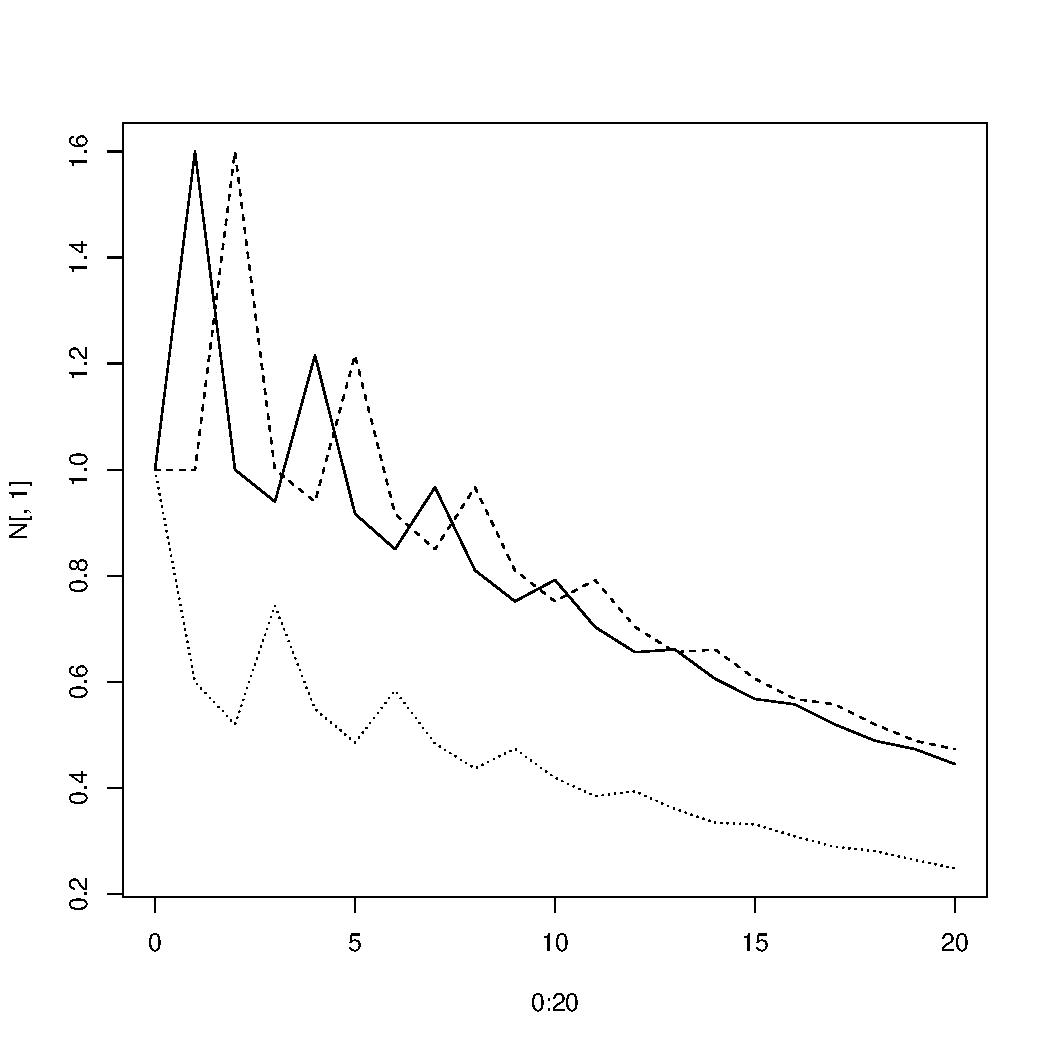
\includegraphics[width=\maxwidth]{figure/plot} 

\end{knitrout}

Exercise 3. Modify this code to add (a) an x-axis label, `time-step',
(b) y-axis label, `state', and (c) legend identifying the different
line types used for the three different states.

%Exercise 1. If \code{X} represents a demographic matrix,
%what is the expected long-term growth rate of the population?
%Is it growing or shrinking?  Copy \code{X} to a new matrix
%\code{Y} and change \code{Y} in some way that leads to 
%a growth rate that is just $<1$, if the original growth
%rate was $>1$, or vice versa.


% maxima
% (%i37) m : matrix([0,f1,f2],[s1,0,0],[0,s2,s3]);

Exercise 4. Show that starting with initial values of either
$\{1,1,1\}$ or $\{1,0,0\}$ gets you to the same state after 100 time
steps (you can either use a \code{for} loop or the \verb+%^%+ operator
from the \code{expm} package), and these states are the same as the
first eigenvector.  Don't forget to normalize!








Download the data file \code{horn.txt} from Avenue (under `Content ->
Data`).

\begin{knitrout}
\definecolor{shadecolor}{rgb}{0.969, 0.969, 0.969}\color{fgcolor}\begin{kframe}
\begin{alltt}
\hlstd{> }\hlstd{f} \hlkwb{<-} \hlkwd{file.choose}\hlstd{()}  \hlcom{## on MacOS or Windows this should open a dialog box}
\end{alltt}
\end{kframe}
\end{knitrout}

\begin{knitrout}
\definecolor{shadecolor}{rgb}{0.969, 0.969, 0.969}\color{fgcolor}\begin{kframe}
\begin{alltt}
\hlstd{> }\hlstd{(X} \hlkwb{<-} \hlkwd{as.matrix}\hlstd{(}\hlkwd{read.table}\hlstd{(}\hlstr{"horn.txt"}\hlstd{)))}
\end{alltt}
\begin{verbatim}
##                   BTA GB SF BG SG WO OK HI TU RM BE
## Big-toothed aspen   3  5  9  6  6  0  2  4  2 60  3
## Gray birch          0  0 47 12  8  2  8  0  3 17  3
## Sassafras           3  1 10  3  6  3 10 12  0 37 15
## Blackgum            1  1  3 20  9  1  7  6 10 25 17
## Sweetgum            0  0 16  0 31  0  7  7  5 27  7
## White oak           0  0  6  7  4 10  7  3 14 32 17
## Red oaks            0  0  2 11  7  6  8  8  8 33 17
## Hickories           0  0  1  3  1  3 13  4  9 49 17
## Tulip tree          0  0  2  4  4  0 11  7  9 29 34
## Red maple           0  0 13 10  9  2  8 19  3 13 23
## Beech               0  0  0  2  1  1  1  1  8  6 80
\end{verbatim}
\end{kframe}
\end{knitrout}

Notice that the row sums are all equal to 100 --- %
these data are in percentages, we want the
\emph{column sums} to be 1:
\begin{knitrout}
\definecolor{shadecolor}{rgb}{0.969, 0.969, 0.969}\color{fgcolor}\begin{kframe}
\begin{alltt}
\hlstd{> }\hlkwd{rowSums}\hlstd{(X)}
\end{alltt}
\begin{verbatim}
## Big-toothed aspen        Gray birch         Sassafras 
##               100               100               100 
##          Blackgum          Sweetgum         White oak 
##               100               100               100 
##          Red oaks         Hickories        Tulip tree 
##               100               100               100 
##         Red maple             Beech 
##               100               100
\end{verbatim}
\begin{alltt}
\hlstd{> }\hlstd{X} \hlkwb{<-} \hlkwd{t}\hlstd{(X)}\hlopt{/}\hlnum{100}  \hlcom{## transpose and divide by 100}
\hlstd{> }\hlkwd{colSums}\hlstd{(X)}
\end{alltt}
\begin{verbatim}
## Big-toothed aspen        Gray birch         Sassafras 
##                 1                 1                 1 
##          Blackgum          Sweetgum         White oak 
##                 1                 1                 1 
##          Red oaks         Hickories        Tulip tree 
##                 1                 1                 1 
##         Red maple             Beech 
##                 1                 1
\end{verbatim}
\end{kframe}
\end{knitrout}

This matrix contains the parameters for a linear model of temporal
changes in the species composition of a forest. The changes in the
abundances of the species depend on the current composition of
species. Therefore, if we start with a forest containing only
big-toothed aspen and nothing else, the composition after one time
step would be,
\begin{knitrout}
\definecolor{shadecolor}{rgb}{0.969, 0.969, 0.969}\color{fgcolor}\begin{kframe}
\begin{alltt}
\hlstd{> }\hlstd{n0} \hlkwb{<-} \hlkwd{numeric}\hlstd{(}\hlkwd{nrow}\hlstd{(X))}
\hlstd{> }\hlstd{n0[}\hlnum{1}\hlstd{]} \hlkwb{<-} \hlnum{1}
\hlstd{> }\hlstd{X} \hlopt \hlstd{n0}
\end{alltt}
\begin{verbatim}
##     [,1]
## BTA 0.03
## GB  0.05
## SF  0.09
## BG  0.06
## SG  0.06
## WO  0.00
## OK  0.02
## HI  0.04
## TU  0.02
## RM  0.60
## BE  0.03
\end{verbatim}
\end{kframe}
\end{knitrout}
The idea here is that big-toothed aspen facilitates the establishment
of certain other species.

Exercise 6* (this will be homework).  Determine the long-run
composition of the forest using a \code{for} loop, the explicit
closed-form eigenvector-based solution, \emph{or} the \verb+%^%+
operator in the \code{exmp} package, and compare it with the dominant
eigenvector (don't forget to normalize!).  Sort the normalized vector
of the long-run composition in decreasing order and produce a bar plot
of the state variable (HINT: type \code{?sort} and \code{?barplot} to
see these help files). The results of a \code{for} loop or the
\verb+%^%+ operator will have names, which will be convenient for your
bar plot). What is the dominant species?  How many species will be
present at frequencies of $>5\%$? Is the origin a stable fixed point
in this model (HINT: What happens if one of the eigenvalues has
modulus of exactly one? Do your best!)



%% \bibliography{bookbib}

\end{document}

